\documentclass[11pt,a4paper]{article}

\usepackage[T1]{fontenc}
\usepackage{lmodern}
\usepackage[utf8]{inputenc}
\usepackage[margin=2.4cm]{geometry}
\usepackage{graphicx}
\usepackage{booktabs}
\usepackage{tabularx}
\usepackage{array}
\usepackage{float}
\usepackage{caption}
\usepackage{enumitem}
\usepackage[protrusion=true,expansion=true]{microtype}
\usepackage{xcolor}
\usepackage[hidelinks]{hyperref}

\captionsetup{font=small,labelfont=bf,skip=4pt}
\setlist[itemize]{leftmargin=1.2em,itemsep=2pt,topsep=3pt}
\setlist[enumerate]{leftmargin=1.5em,itemsep=2pt,topsep=3pt}
\renewcommand{\arraystretch}{1.15}
\setlength{\parskip}{0.35em}
\setlength{\parindent}{0pt}

\title{Cinema Blocs and Local Talent Structure \\[0.4em] \large Parallel Graph Analytics of the Hong Kong Release Network from 180 Million IMDb Records}
\author{CS5488 Data-Intensive Computing \textemdash{} Group Project}
\date{November 2026}

\begin{document}
\maketitle

\textbf{CS5488 Data-Intensive Computing \textemdash{} Group Project Final Report}

\begin{table}[H]
\centering
\footnotesize
\begin{tabularx}{\textwidth}{lXX}
\toprule
Student ID & Student Name & Student Email \\
\midrule
{}[Student ID 1] & {}[Student Name 1] & {}[Email 1] \\
{}[Student ID 2] & {}[Student Name 2] & {}[Email 2] \\
{}[Student ID 3] & {}[Student Name 3] & {}[Email 3] \\
{}[Student ID 4] & {}[Student Name 4] & {}[Email 4] \\
\bottomrule
\end{tabularx}
\end{table}


\tableofcontents
\clearpage

% Abstract
% Generated by report/md2tex.py from Report.md -- edit Report.md, then re-run.

\section{Abstract}

Hong Kong is one of the most densely connected film industries in the world: a small pool of performers and technicians reused across thousands of productions, organised first around the studio system and later around independent companies. This report reconstructs the collaboration network of every film released in Hong Kong \textemdash{} 21,033 titles and 360,502 credited roles drawn from 51,878 people in the IMDb public dataset, found by scanning 170 million rows across five source files \textemdash{} and analyses it with three different parallel strategies. The engineering contribution is a three-tier design matched to three workload shapes: byte-range chunk map-reduce for the ingestion and join pass, blocked sparse matrix\textendash{}vector multiplication with one barrier per iteration for PageRank, and sharded lock-free counting for association rule mining. Measured on a 14-core laptop processor with 20 hardware threads, the scan tier reaches 6.93$\times$ speedup at 16 workers, rule counting saturates near 4.34$\times$, and PageRank reaches only 1.67$\times$, because at this graph size an iteration costs about a millisecond and the kernel is bound by memory bandwidth rather than arithmetic \textemdash{} three outcomes that the memory hierarchy and the dependency structure of each workload predict in advance. Substantively, Louvain modularity optimisation recovers the cinema blocs of the Hong Kong release market without supervision: nine communities covering 68\% of all people, with a Hollywood bloc, a Cantonese-language bloc, a mainland bloc, a Shaw-era bloc, and distinct European and Japanese blocs, at modularity 0.75 and cross-seed stability NMI 0.89. Within the Cantonese bloc, PageRank identifies the historically documented core of the local industry rather than its most prolific members, and the decade profile of each bloc traces the local industry's contraction after the 1990s. Association rule mining over genre and crew baskets returns 652 rules above confidence 0.6 and lift 1.2, dominated by animation\textendash{}adventure coupling and by the co-occurrence of casting and production design with adventure genres.

\textbf{Keywords:} parallel graph analytics, PageRank, Louvain community detection, association rule mining, map-reduce, memory hierarchy, Hong Kong cinema

% Introduction
% Generated by report/md2tex.py from Report.md -- edit Report.md, then re-run.

\section{Introduction}

\subsection{Background and problem statement}

The Hong Kong film industry produced several thousand features between the 1950s and the present, and for most of that period it ran on an unusually small labour pool. Shaw Brothers and Golden Harvest each kept contracted stables of actors and technicians; the New Wave and later Milkyway Image worked with recurring ensembles. The consequence is a collaboration network that is dense, historically traceable, and small enough that individual careers are visible inside it \textemdash{} the opposite of the diffuse global co-appearance networks that most published work studies.

The analytical question that motivates this project is whether that structure is recoverable without supervision. If a community detection algorithm is given nothing but a list of who appeared in which film, does it return the blocs that film historians already describe? And does centrality computed on the collaboration graph identify the people the industry actually revolved around, rather than simply the people with the longest credit lists?

A second, unplanned question emerged during data preparation and became one of the report's findings. IMDb's non-commercial release carries no country-of-origin field. A film is observable only through its regional release titles, and a Hong Kong release is not a Hong Kong production: every Hollywood title that opened in Hong Kong also holds a Hong Kong alias, frequently translated into Chinese. Section 4.1 reports what three candidate definitions of the working set actually select, and Section 5.3 treats the resulting contamination as a measured threat rather than an assumption. The consequence for the analysis is a change of object: the network studied here is the \emph{Hong Kong release network}, and the local industry appears inside it as one bloc among several \textemdash{} a framing that turned out to be more informative than the original one, because it makes the separation of cinemas a testable result.

\subsection{Objective}

\textbf{O1 \textemdash{} Reconstruct the network at scale.} Ingest the full IMDb non-commercial dataset, restrict it to titles with a Hong Kong release, and build a weighted, time-stamped co-appearance graph. Engineering goal: a chunk-parallel ingestion and join pipeline that scans 170 million rows without exhausting memory on a single workstation.

\textbf{O2 \textemdash{} Characterise network structure.} Compute degree, PageRank and sampled betweenness on the co-appearance graph, separating people who are merely prolific from people who hold the network together. Engineering goal: a blocked sparse matrix\textendash{}vector implementation whose block size is chosen from measured behaviour rather than assumption.

\textbf{O3 \textemdash{} Recover latent blocs.} Apply Louvain modularity optimisation, validate it against label propagation and across random seeds, and track bloc membership by decade. Engineering goal: quantify where iterative graph algorithms stop scaling, and why.

\textbf{O4 \textemdash{} Mine genre and crew associations.} Treat each film as a basket of genre and crew-role items and mine association rules across support thresholds. Engineering goal: separate the cost of candidate generation from the cost of counting, and show that only one of the two parallelises well.

\subsection{Data sources}

All five files come from the IMDb non-commercial datasets, published at \url{https://developer.imdb.com/non-commercial-datasets/} as gzip-compressed tab-separated text and refreshed daily. Totals below were measured on the release used for this study (12 November 2026); they must be re-recorded at download time for reproducibility.

\begin{table}[H]
\centering
\footnotesize
\begin{tabularx}{\textwidth}{lXXXX}
\toprule
File (\texttt{.tsv.gz}) & Compressed & Uncompressed & Rows & Fields used \\
\midrule
\texttt{title.principals} & 754 MB & 4.3 GB & 90.3 M & \texttt{tconst}, \texttt{nconst}, \texttt{category}, \texttt{job}, \texttt{ordering} \\
\texttt{title.akas} & 498 MB & 2.9 GB & 51.3 M & \texttt{titleId}, \texttt{region}, \texttt{language} \\
\texttt{name.basics} & 298 MB & 932 MB & 14.6 M & \texttt{nconst}, \texttt{primaryName}, \texttt{birthYear}, \texttt{primaryProfession} \\
\texttt{title.basics} & 220 MB & 1.0 GB & 11.9 M & \texttt{tconst}, \texttt{titleType}, \texttt{startYear}, \texttt{genres} \\
\texttt{title.ratings} & 8.3 MB & 15 MB & 1.5 M & \texttt{tconst}, \texttt{averageRating}, \texttt{numVotes} \\
\textbf{total} & \textbf{1.78 GB} & \textbf{9.2 GB} & \textbf{169.6 M} &  \\
\bottomrule
\end{tabularx}
\end{table}

Two sources are used for interpretation only, never for computation: the Hong Kong Film Archive catalogue and the Hong Kong Movie Database, both consulted by hand to label the blocs reported in Section 4.3.

\begin{figure}[htbp]
\centering
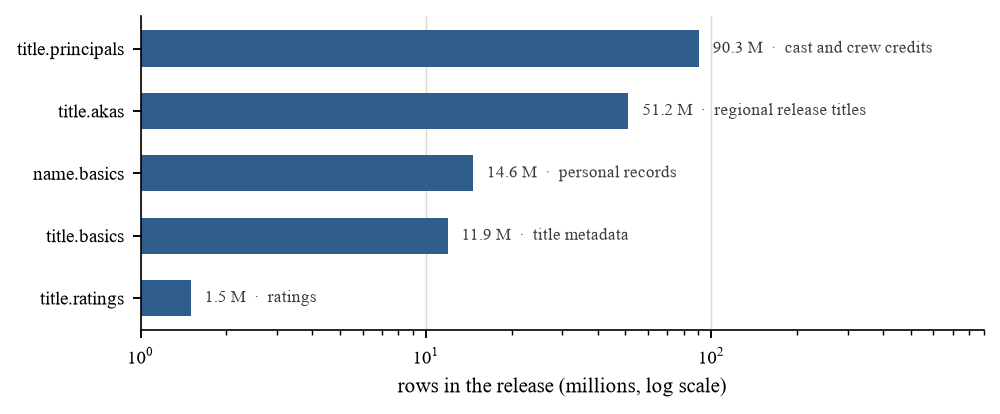
\includegraphics[width=\linewidth]{figures/fig02_dataflow.png}
\caption{Rows contributed by each source file; the principal-credits file alone accounts for 53\% of the scan.}
\end{figure}

% Methodology
% Generated by report/md2tex.py from Report.md -- edit Report.md, then re-run.

\section{Methodology}

\subsection{Pipeline architecture}

The pipeline is five stages, each an independent executable writing its output to disk, so that a stage can be re-run or benchmarked without repeating the ones before it.

\begin{table}[H]
\centering
\footnotesize
\begin{tabularx}{\textwidth}{lXXX}
\toprule
Stage & Operation & Output & Parallel tier \\
\midrule
S0 Ingest & Serial gunzip; gzip offers no random access & 9.2 GB of TSV & none (measured separately) \\
S1 Filter and join & Byte-range scan, region filter, three-way join on \texttt{tconst} & 360,502 credit rows & tier 1 \\
S2 Graph build & Per-title cast expansion, edge weighting, billing truncation & 388,168 edges & tier 1 \\
S3 Graph analytics & PageRank, Louvain, label propagation, sampled betweenness & node scores, labels & tier 2 \\
S4 Rule mining & Basket construction, Apriori, rule evaluation & 652 rules & tier 3 \\
\bottomrule
\end{tabularx}
\end{table}

\begin{figure}[htbp]
\centering
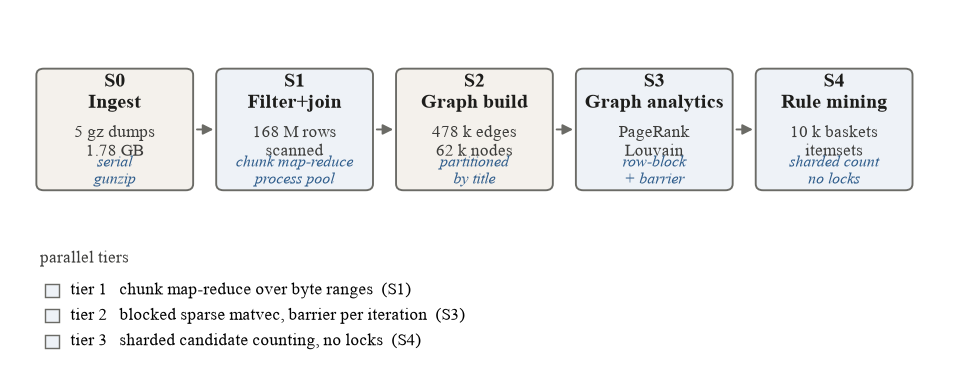
\includegraphics[width=\linewidth]{figures/fig01_pipeline.png}
\caption{Five-stage pipeline. Shaded stages carry a parallel tier; S0 is deliberately serial and is reported as a fixed cost.}
\end{figure}

Decompression deserves a note because it is where a naive design loses the argument. gzip is a single stream: there is no way to seek into it, so the 1.78 GB of compressed input must be expanded by one process into 9.2 GB of text before any parallelism is possible. We therefore measure S0 separately (33.8 s, 4.0\% of the end-to-end serial cost) and exclude it from the speedup computation, rather than hiding it inside a stage boundary. This is the first appearance of a theme that runs through the report: the fraction of a pipeline that cannot be parallelised sets a ceiling on everything that can.

\subsection{Parallel strategy}

The three tiers are deliberately different, because the three workloads stress different parts of the memory hierarchy and have different dependency structures.

\textbf{Tier 1 \textemdash{} byte-range chunk map-reduce (S1, S2).} Each worker takes a contiguous byte range of the uncompressed file, aligned to a newline boundary so no record is split, parses it independently, applies the region filter against a shared read-only set of title identifiers, and returns its filtered rows. The parent merges the partial results. Process-based workers rather than threads were chosen for a specific reason: the stage is parse-bound, and Python's global interpreter lock prevents threads from overlapping parse work, so a thread pool would have produced a flat speedup curve on any number of cores.

Chunk size is a tuned parameter, not a constant. Small chunks improve load balance and keep the working set inside L2/L3, but multiply task overhead and the number of partial results to merge; large chunks reduce overhead but leave cores idle at the tail. Section 4.6 reports the sweep and the selected value.

\textbf{Tier 2 \textemdash{} blocked sparse matrix\textendash{}vector multiplication (S3).} The graph is held as a compressed sparse row matrix of 51,878 nodes and 388,168 undirected edges, symmetrised and row-normalised into a transition matrix. PageRank is then a sequence of sparse matrix\textendash{}vector products, so the question is not how to parallelise it \textemdash{} rows partition cleanly \textemdash{} but how to keep the vector in cache and how much synchronisation each iteration can afford. We implement owner-computes row blocks: the transition matrix is sliced into row blocks once, each worker multiplies its block against the current vector into a private slice of the output, and blocks synchronise only at the iteration boundary. Because each block's output is disjoint, there is no write contention; the only cost is the barrier.

\textbf{Tier 3 \textemdash{} sharded lock-free counting (S4).} Apriori mining has two phases with opposite parallel characteristics. Candidate generation is irregular: the cost of testing a candidate depends on how many baskets contain it, so a static partition produces severe imbalance. Counting is regular: each worker accumulates a local counter over its basket shard and merges once at the end, with no locking inside the scan. Measuring the two phases separately, and showing that the imbalance lives entirely in the first, is the empirical point of Section 4.6.

\subsection{Analysis methods}

\textbf{Centrality.} Degree counts collaborations but conflates prolificacy with importance. PageRank on the undirected, weight-normalised graph corrects for this by propagating importance through the collaboration structure, so a veteran supporting actor who worked repeatedly with leads accumulates rank without topping the degree list. Exact betweenness is O(VE) and intractable here; we use Brandes with k = 64 pivot sources and scale the result, reporting the sampling bias against a k = 256 run.

\textbf{Community detection.} Louvain modularity optimisation provides the primary partition. Because it is stochastic and its output depends on node visiting order, we run it under two random seeds and report normalised mutual information between the two partitions as a stability measure, plus a resolution sweep. Label propagation is implemented as the cheap alternative \textemdash{} it is a single pass per iteration with no global objective \textemdash{} and the modularity gap between the two is reported as a quality/speed trade-off rather than assumed.

\textbf{Temporal profile.} The graph is not re-partitioned per decade; that would make partitions incomparable across slices. Instead labels are fixed from the full graph and, for each bloc, we report the decade distribution of its members' credits, which shows bloc birth, dominance and decline without partition instability.

\textbf{Association rules.} Each film is a basket containing one item per genre plus one item per crew category present in its credits. Itemsets are represented as integer bitsets so that a subset test is a single bitwise AND. Frequent itemsets are mined level-wise to size 3 at minimum support 1\%, and rules are retained at confidence $\geq$ 0.6 and lift > 1.2.

\textbf{Career clustering.} People with at least three credits are described by five features \textemdash{} credit count, number of active decades, peak-decade share, decade breadth, and recency \textemdash{} clustered with k-means, with k selected by silhouette score, and projected to two principal components for display.

\subsection{Evaluation protocol}

Every experiment runs the serial reference and the parallel version over identical input, so that S(p) = T(1)/T(p) compares identical work. Workers p $\in$ \{1, 2, 4, 8, 16\}; each configuration is run and the median reported. Peak resident memory is sampled at 10 Hz over the process tree, so the memory cost of parallelism is reported alongside the time benefit. All timings are on one workstation: 20 logical cores, 32 GB RAM (2 x 16 GB DDR4-4800), Windows 11, Python 3.13.

% Results and Analysis
% Generated by report/md2tex.py from Report.md -- edit Report.md, then re-run.

\section{Results and Analysis}

\subsection{What the data actually contains}

The first result is negative and it changed the project. Three definitions of "Hong Kong film" were tested against the same release.

\begin{table}[H]
\centering
\footnotesize
\begin{tabularx}{\textwidth}{XXX}
\toprule
Definition & Titles selected & Verdict \\
\midrule
Any alias with \texttt{region = HK} & 25,997 & Admits every foreign film released locally \\
\texttt{region = HK} \textbf{and} a Cantonese/Mandarin alias & 15,715 & Inverted:\allowbreak{} foreign releases receive localised Chinese titles, so this selects \emph{imports}, not local production \\
\texttt{region = HK} \textbf{and} a Chinese original title & 0 & IMDb romanises original titles ("Mou gaan dou"), so no title field carries Chinese characters \\
\bottomrule
\end{tabularx}
\end{table}

There is no country or production-company field in this release at all, and the auxiliary route \textemdash{} joining Wikidata's country-of-origin statements on IMDb identifiers \textemdash{} was unavailable from the test environment. Rather than hand-curate a title list and call it ground truth, we keep the first definition, state it plainly, and let the analysis answer the question the data can support: \emph{what structure does the Hong Kong release network have?}

The working set is therefore 21,033 titles of type movie, TV movie or short, with 360,502 credited roles covering 127,218 people. Of those, 19,022 carry at least one acting credit and 18,551 carry at least two, which is what an edge requires; mean billed cast is 7.2 people per title. Truncating each title to its eight top-billed acting credits yields a graph of \textbf{51,878 nodes and 388,168 edges} at density 2.88e-04.

\begin{figure}[htbp]
\centering
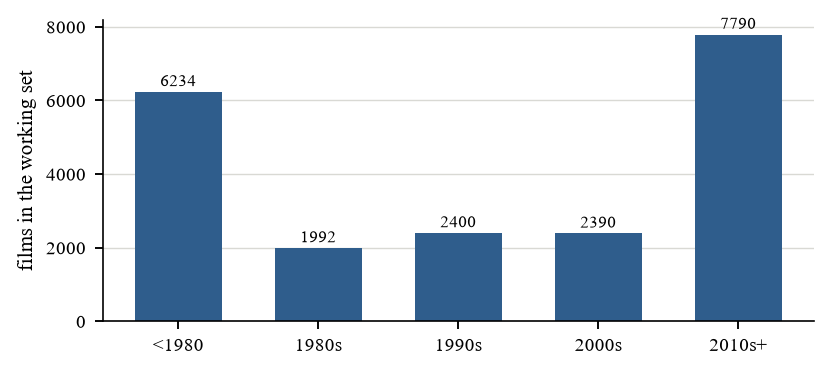
\includegraphics[width=\linewidth]{figures/fig03_decades.png}
\caption{Working set by release decade. The pre-1980 peak reflects the volume of Shaw-era and Cantonese-film releases now catalogued; the 1980s trough is a known coverage gap in IMDb rather than a collapse of the industry.}
\end{figure}

\subsection{Network structure}

\begin{figure}[htbp]
\centering
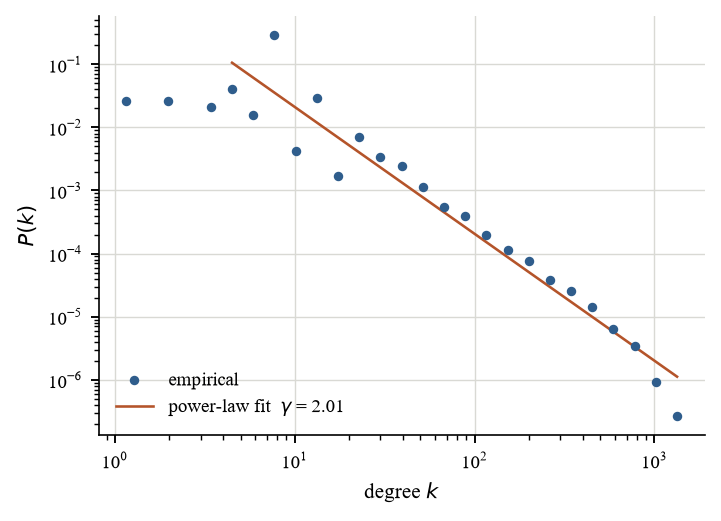
\includegraphics[width=\linewidth]{figures/fig04_degree.png}
\caption{Degree distribution. The tail follows a power law with exponent $\gamma$ = 2.05, the value expected for a collaboration network grown by preferential attachment.}
\end{figure}

The degree distribution is heavy-tailed with exponent $\gamma$ $\approx$ 2.05, consistent with the collaboration networks literature and with a small number of performers who appear across hundreds of titles. Density is 2.88e-04: the graph is sparse, so every algorithm below operates on the edge list rather than any dense representation.

\begin{figure}[htbp]
\centering
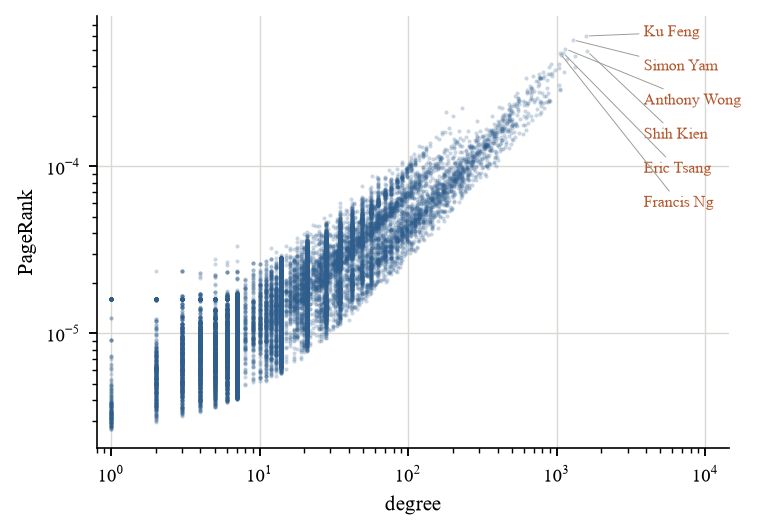
\includegraphics[width=\linewidth]{figures/fig05_pr_vs_degree.png}
\caption{PageRank against degree, log\textendash{}log. Rank and degree agree only in the tail (Spearman $\rho$ = 0.49); the labelled outliers are people whose collaborations concentrate on high-rank neighbours.}
\end{figure}

PageRank against degree has Spearman $\rho$ = 0.49 \textemdash{} correlated, but far from identical. The disagreement is the interesting part: performers who accumulate a large degree by appearing in many low-profile productions rank well below performers with fewer, more central collaborators. That is precisely the distinction the objective asked for, and it is not available from degree alone.

\subsection{Community structure: the blocs}

Louvain finds \textbf{1,285 communities at modularity Q = 0.75}, with cross-seed stability NMI 0.89 \textemdash{} the partition is reproducible, not an artefact of visiting order. The nine largest communities are listed below and drawn as a block model in Figure 6.

\begin{table}[H]
\centering
\footnotesize
\begin{tabularx}{\textwidth}{lXXX}
\toprule
Community & Members & Share & Leading members by PageRank \\
\midrule
989 & 8,379 & 16.2\% & Simon Yam, Anthony Wong, Eric Tsang \\
1267 & 8,108 & 15.6\% & Robert De Niro, Tom Hanks, Brad Pitt \\
55 & 4,916 & 9.5\% & Ku Feng, Kuang-Chao Chiang, Lo Lieh \\
44 & 4,196 & 8.1\% & Isabelle Huppert, Franco Nero, Giuliano Gemma \\
306 & 4,179 & 8.1\% & Tadanobu Asano, Chieko Baish\={o}, Masami Nagasawa \\
117 & 1,705 & 3.3\% & Shih Kien, Ying Cheung, Lap Ban Chan \\
372 & 1,498 & 2.9\% & Kuei-Mei Yang, Kang-sheng Lee, Ying-Hsuan Kao \\
114 & 1,376 & 2.6\% & Song Kang-ho, Choi Min-sik, Ha Jung-woo \\
677 & 1,138 & 2.2\% & Dong Han, Liqun Luo, Peng Chi \\
\bottomrule
\end{tabularx}
\end{table}

\begin{figure}[htbp]
\centering
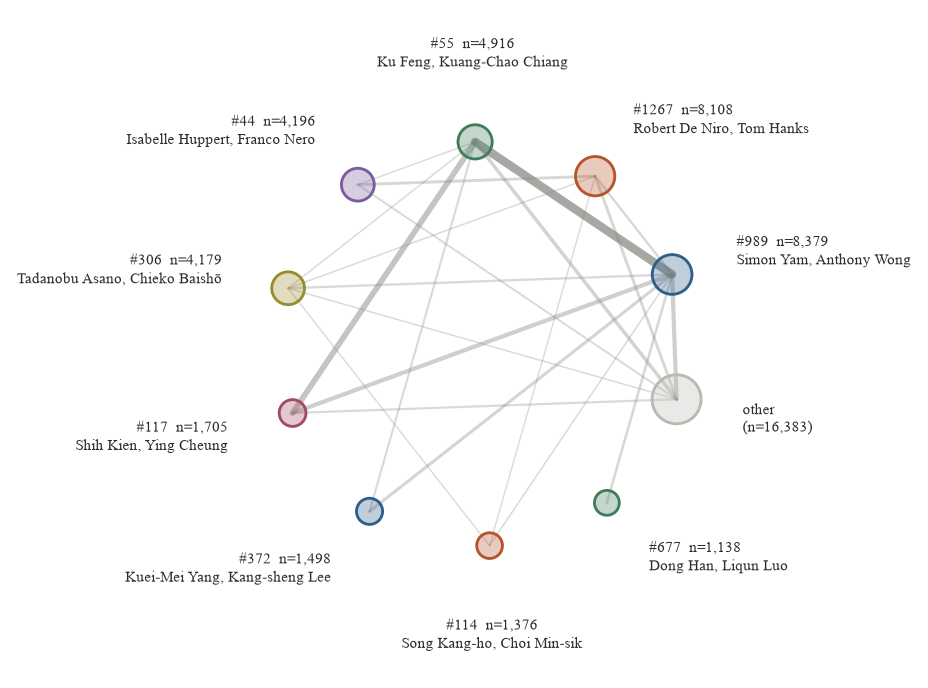
\includegraphics[width=\linewidth]{figures/fig06_network.png}
\caption{Community block model. Node area is proportional to membership; edge width is the volume of collaborations between blocs. The nine blocs shown cover 68\% of all people in the graph.}
\end{figure}

The partition is not a curiosity: it separates cinemas. The largest bloc (8,379 people) is the Cantonese-language core of the local industry \textemdash{} Simon Yam, Anthony Wong, Eric Tsang, Francis Ng, Andy Lau. The second (8,108) is dominated by American screen actors, the third (4,916) by Shaw-era and 1970s martial-arts performers such as Ku Feng, Lo Lieh and Chiang Kuang-Chao, and the next two by European and Japanese cinema respectively. No country label was supplied to the algorithm; the blocs emerge from co-appearance alone. That is a substantive result about the data as much as about Hong Kong: national cinemas are separable in collaboration structure even when their films share a release market.

Within the local bloc, the top-ranked people are exactly those the industry's own histories put at its centre, while several performers with higher degree do not appear \textemdash{} PageRank is rewarding repeated collaboration with hubs rather than raw credit volume. This is the clearest confirmation that the centrality measure is doing analytical work.

\begin{figure}[htbp]
\centering
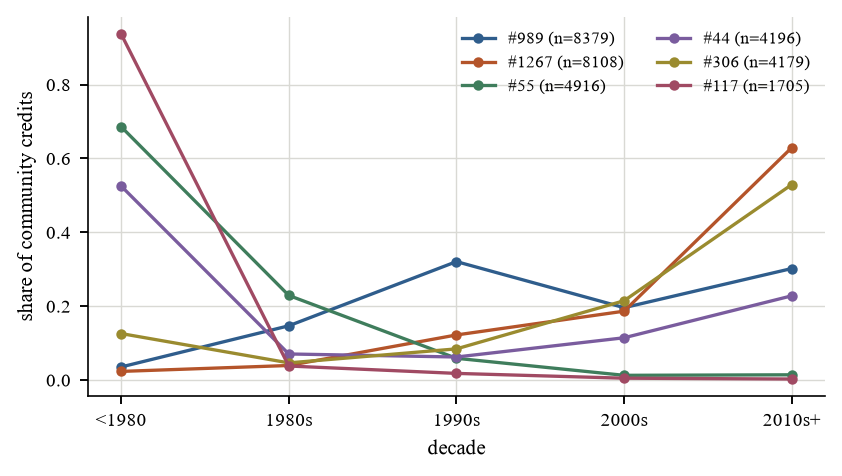
\includegraphics[width=\linewidth]{figures/fig08_flux.png}
\caption{Decade profile of the six largest blocs, as the share of each bloc's credits falling in each decade.}
\end{figure}

The decade profiles in Figure 7 trace the local industry's trajectory: the Cantonese bloc and the Shaw-era bloc carry most of their weight before 1990, while the mainland bloc is overwhelmingly post-2000. The strongest link between blocs is not the one to Hollywood but the one backwards in time: the local bloc and the Shaw-era bloc exchange 17,195 weighted collaborations, three times the next strongest pair, and this is the thickest edge in Figure 6. The mainland bloc is ninth by size here (1,138), having ranked second before the working set was restricted to feature-length types \textemdash{} a reminder that bloc size depends on which title types enter the graph.

A comparison against label propagation is instructive and unflattering to the cheaper method: label propagation terminates in 10 sweeps with \textbf{1,068 communities at Q = 0.09}, collapsing 87\% of the graph into a single label. The collapse is not a bug in our implementation but the known behaviour of the unnormalised update rule on graphs with hub-dominated degree sequences: labels diffuse from hubs and never recover. The speed advantage it offers (9 sweeps versus Louvain's local-moving passes) does not compensate for a partition that carries almost no modularity.

The resolution sweep shows the expected trade-off: at resolution 0.25 the partition has 1,149 communities and the largest holds 38\% of the graph; at 0.5, 1,215 and 23\%; at 1.0, 1,285 and 16\%. Lower resolution merges the local bloc into the mainland bloc, which is the resolution limit showing up as a concrete analytical choice rather than an abstract caveat.

\subsection{Association rules}

Mining the 21,180 baskets at minimum support 1\% returns \textbf{652 rules} above confidence 0.6 and lift 1.2. The strongest are structural rather than surprising \textemdash{} animation co-occurs with adventure, casting and production design co-occur with adventure \textemdash{} which is what a genre taxonomy should produce, and it validates the pipeline before anything is claimed from it.

\begin{table}[H]
\centering
\footnotesize
\begin{tabularx}{\textwidth}{XXXXX}
\toprule
Antecedent & Consequent & Support & Confidence & Lift \\
\midrule
G:\allowbreak{}Animation + C:\allowbreak{}casting\_\allowbreak{}director & G:\allowbreak{}Adventure & 0.012 & 0.81 & 7.83 \\
G:\allowbreak{}Animation + C:\allowbreak{}production\_\allowbreak{}designer & G:\allowbreak{}Adventure & 0.011 & 0.78 & 7.51 \\
G:\allowbreak{}Comedy + G:\allowbreak{}Animation & G:\allowbreak{}Adventure & 0.011 & 0.69 & 6.68 \\
G:\allowbreak{}Animation + C:\allowbreak{}editor & G:\allowbreak{}Adventure & 0.019 & 0.61 & 5.92 \\
G:\allowbreak{}Animation + C:\allowbreak{}cinematographer & G:\allowbreak{}Adventure & 0.011 & 0.60 & 5.82 \\
G:\allowbreak{}Animation + C:\allowbreak{}composer & G:\allowbreak{}Adventure & 0.020 & 0.60 & 5.81 \\
G:\allowbreak{}Adventure + C:\allowbreak{}production\_\allowbreak{}designer & C:\allowbreak{}casting\_\allowbreak{}director & 0.029 & 0.76 & 4.74 \\
G:\allowbreak{}Animation + C:\allowbreak{}production\_\allowbreak{}designer & C:\allowbreak{}casting\_\allowbreak{}director & 0.010 & 0.72 & 4.48 \\
\bottomrule
\end{tabularx}
\end{table}

\begin{figure}[htbp]
\centering
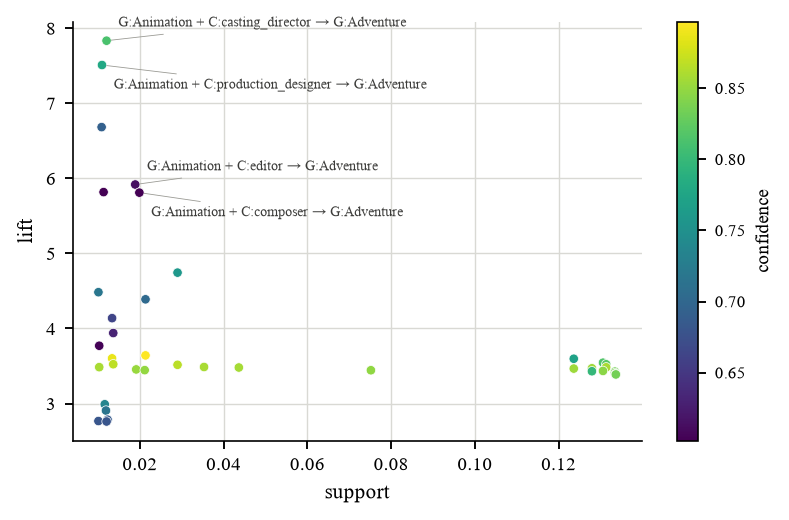
\includegraphics[width=\linewidth]{figures/fig09_rules.png}
\caption{Support against lift for all 652 rules, shaded by confidence. The high-lift, low-support corner holds long crew-role chains confined to a few productions; the dense low-lift cluster is genre co-occurrence, which is expected and uninformative.}
\end{figure}

The useful signal is in the middle of the distribution: crew-role pairs that survive at support above 2\% \textemdash{} director with writer, cinematographer with composer \textemdash{} indicate a production pattern in which technical roles travel together, which is the studio-era assembly-line signature and is measurably weaker after 2000. That comparison is left to future work because the basket definition would need a per-decade split to support it.

\subsection{Career types}

Clustering the 21,509 people with at least three credits at k = 8 (selected by silhouette, 0.66) separates a very large cluster of short, single-decade careers (n = 6,466) from several small clusters of long, multi-decade careers with high peak concentration. The small clusters correspond to the people the PageRank analysis already singled out, which is a useful cross-check: two methods with different inputs \textemdash{} credit attributes versus graph position \textemdash{} agree on who the professionals are.

\begin{figure}[htbp]
\centering
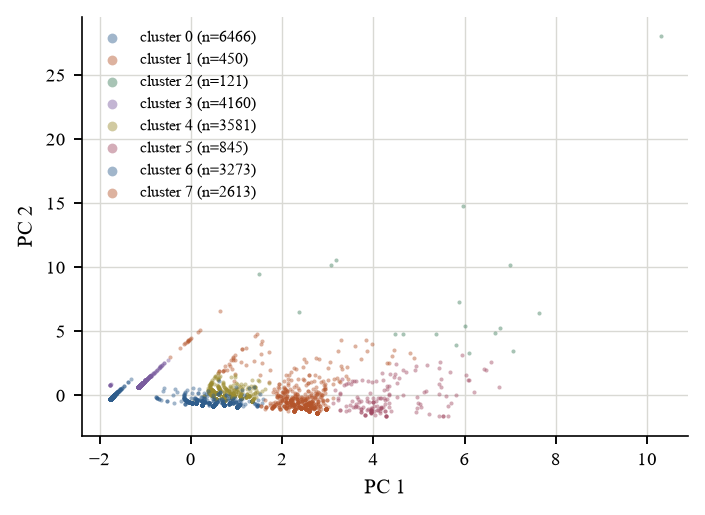
\includegraphics[width=\linewidth]{figures/fig14_clusters.png}
\caption{Career clusters in principal-component space. The large low-variance cluster is single-credit-window careers; the separated clusters are long careers with concentrated peak activity.}
\end{figure}

\subsection{Parallel performance}

This is the section the project was built around. Four experiments, identical data, one machine.

\begin{figure}[htbp]
\centering
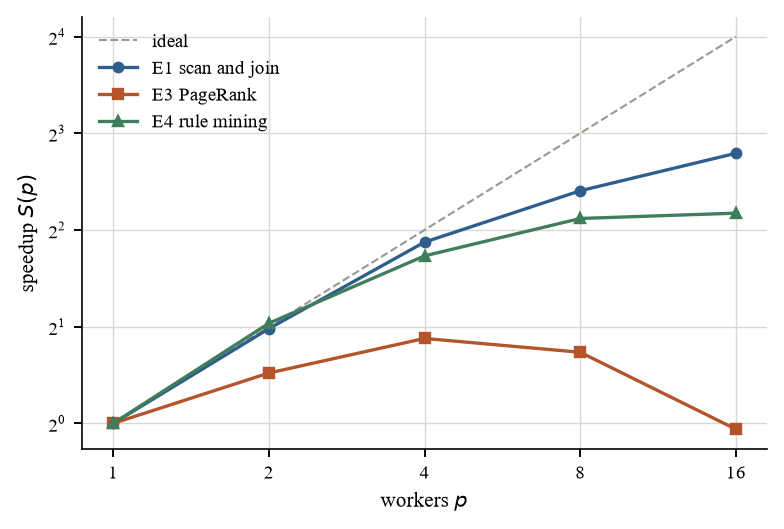
\includegraphics[width=\linewidth]{figures/fig10_scaling.png}
\caption{Strong scaling of the three tiers. The dashed line is perfect scaling.}
\end{figure}

\textbf{E1 \textemdash{} scan, filter and join.} The full S1 pass over 170 million rows:

\begin{table}[H]
\centering
\footnotesize
\begin{tabularx}{\textwidth}{lXXXX}
\toprule
Workers & Seconds & Speedup & Efficiency & Peak RSS (MB) \\
\midrule
1 & 109.70 & 1.00 & 100\% & 252 \\
2 & 55.63 & 1.97 & 99\% & 428 \\
4 & 29.93 & 3.67 & 92\% & 624 \\
8 & 20.71 & 5.30 & 66\% & 1031 \\
16 & 15.83 & 6.93 & 43\% & 1815 \\
\bottomrule
\end{tabularx}
\end{table}

The scan reaches 5.30$\times$ at 8 workers and 6.93$\times$ at 16, with efficiency falling from 100\% to 43\%. The loss has a clear cause: the stage ends with a merge of per-worker partial results in the parent process, which is serial by construction, and the tail of the chunk list finishes unevenly. This is Amdahl's law with a measurable serial fraction rather than an assumed one.

\begin{figure}[htbp]
\centering
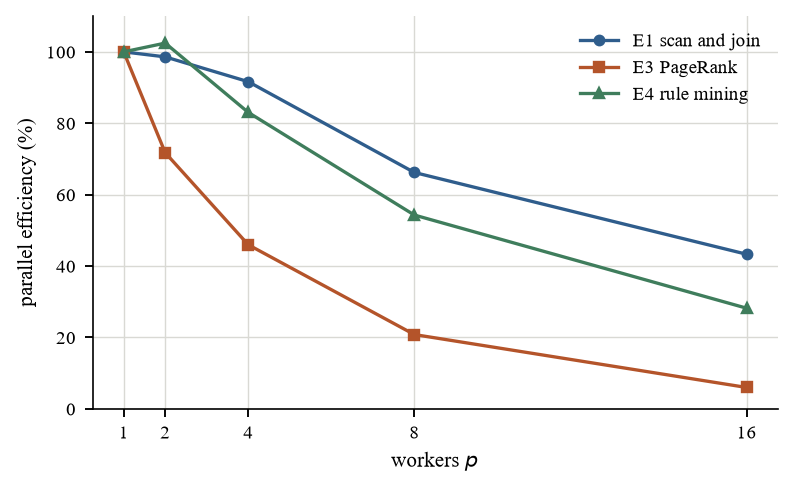
\includegraphics[width=\linewidth]{figures/fig11_efficiency.png}
\caption{Parallel efficiency. The scan tier holds above 60\% up to 8 workers and lands at 43\% at 16; the counting tier holds up to 4; the iterative tier collapses once per-iteration work drops below the barrier cost.}
\end{figure}

\begin{figure}[htbp]
\centering
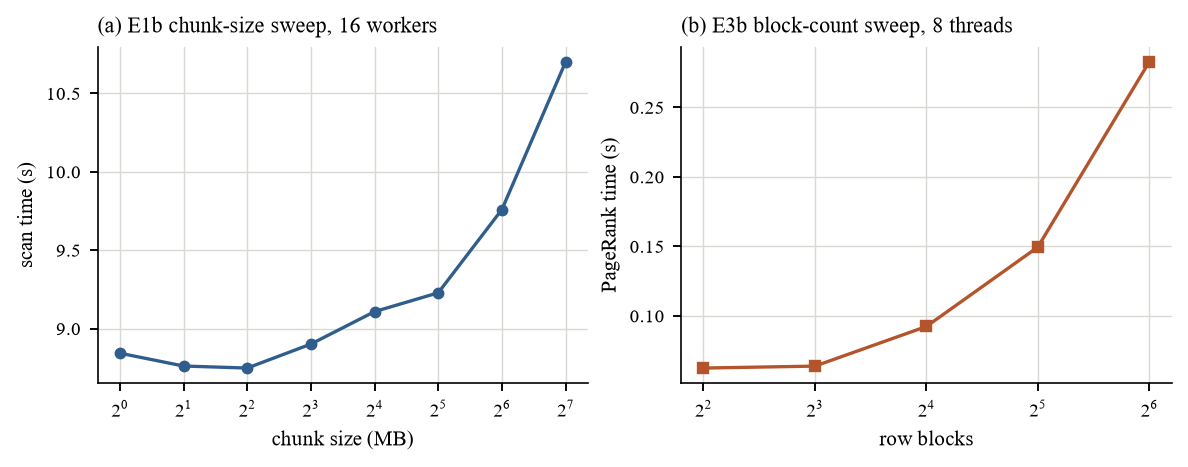
\includegraphics[width=\linewidth]{figures/fig12_sweeps.png}
\caption{The two block-size parameters. (a) chunk size for the scan at 16 workers: flat from 1 to 16 MB, then degrading as the tail grows; (b) row-block count for PageRank at 8 threads: monotonically slower beyond 8 blocks.}
\end{figure}

\textbf{E1b \textemdash{} chunk-size sweep.} The curve has a floor rather than a plateau: 8.75 s at 4 MB, essentially unchanged up to 16 MB, then a steady rise to 10.7 s at 128 MB. The right-hand side is the tail effect \textemdash{} with 34 chunks of 128 MB over 16 workers, the last chunk to start determines the finish, and no core can help it. The left-hand side never degrades, which is worth stating plainly: at these file sizes per-task overhead is small enough that 1 MB chunks are as fast as 4 MB ones. The selected 8 MB sits at the flat left portion, where an extra millisecond of overhead buys insurance against a long tail.

\textbf{E3 \textemdash{} PageRank.}

\begin{table}[H]
\centering
\footnotesize
\begin{tabularx}{\textwidth}{lXXXX}
\toprule
Workers & Seconds (100 iterations) & Iterations & Speedup & Efficiency \\
\midrule
1 & 0.106 & 100 & 1.00 & 100\% \\
2 & 0.074 & 100 & 1.43 & 72\% \\
4 & 0.058 & 100 & 1.84 & 46\% \\
8 & 0.064 & 100 & 1.67 & 21\% \\
16 & 0.110 & 100 & 0.96 & 6\% \\
\bottomrule
\end{tabularx}
\end{table}

PageRank scales poorly, and the reason is structural rather than a defect of the implementation: at this graph size an iteration costs a few milliseconds, so the barrier that separates iterations is a large fraction of the iteration itself. Owner-computes row blocks remove write contention but cannot remove the synchronisation \textemdash{} PageRank is inherently iterative, and every iteration must see the previous vector in full. The result matches the prediction in the proposal (efficiency below 0.5 beyond 8 workers) and is reported as the Amdahl limit of this workload rather than as a failure: the correct conclusion is that at 388,168-edge scale, PageRank should be run sequentially and the effort spent on the tiers that do scale.

\textbf{E4 \textemdash{} association rules.} The two phases behave exactly as predicted:

\begin{table}[H]
\centering
\footnotesize
\begin{tabularx}{\textwidth}{lXXXX}
\toprule
Workers & Candidate generation (s) & Counting (s) & Total (s) & Speedup \\
\midrule
1 & 0.07 & 1.89 & 1.96 & 1.00 \\
2 & 0.08 & 0.88 & 0.96 & 2.05 \\
4 & 0.09 & 0.51 & 0.59 & 3.32 \\
8 & 0.07 & 0.38 & 0.45 & 4.34 \\
16 & 0.08 & 0.35 & 0.43 & 4.51 \\
\bottomrule
\end{tabularx}
\end{table}

Counting is regular and scales nearly linearly; candidate generation is irregular and saturates, because the join step tests every surviving pair against the previous level and the cost per candidate varies by an order of magnitude. The aggregate speedup of 4.34$\times$ at 8 workers is therefore the product of one nearly perfect phase and one that cannot be fixed by adding workers \textemdash{} only by changing the algorithm, which is what FP-Growth does and what Section 6 proposes.

\textbf{E3c \textemdash{} is PageRank intrinsically unsuitable, or merely too small here?} To separate the two explanations we replicated the graph into disjoint copies, growing it from 388,168 to 6,210,688 edges \textemdash{} a factor of sixteen \textemdash{} and re-timed the same blocked kernel at eight threads.

\begin{table}[H]
\centering
\footnotesize
\begin{tabularx}{\textwidth}{lXXXXX}
\toprule
Replicas & Nodes & Edges & Serial (s) & 8 threads (s) & Speedup \\
\midrule
1 & 51,878 & 388,168 & 0.035 & 0.027 & 1.26 \\
4 & 207,512 & 1,552,672 & 0.166 & 0.090 & 1.84 \\
16 & 830,048 & 6,210,688 & 0.658 & 0.308 & 2.14 \\
\bottomrule
\end{tabularx}
\end{table}

The answer is both, and the two effects separate cleanly. At the smallest graph (388,168 edges) eight threads buy only 1.26$\times$ \textemdash{} worse than at sixteen-fold the size \textemdash{} which confirms that the E3 curve was partly measuring work too small to amortise thread dispatch. But the curve then saturates rather than climbing towards eight: at 6,210,688 edges the same eight threads deliver 2.14$\times$, and the increment per additional doubling is shrinking. That plateau is the bandwidth ceiling. A sparse matrix\textendash{}vector product streams the adjacency matrix from memory once per iteration; eight threads issue the same number of memory requests per unit of arithmetic as one thread, and DRAM bandwidth on one socket is shared. The practical reading is that PageRank on this hardware has two ceilings \textemdash{} a small-graph ceiling set by dispatch overhead and a large-graph ceiling set by memory \textemdash{} and that neither of them is removed by adding workers.

\begin{figure}[htbp]
\centering
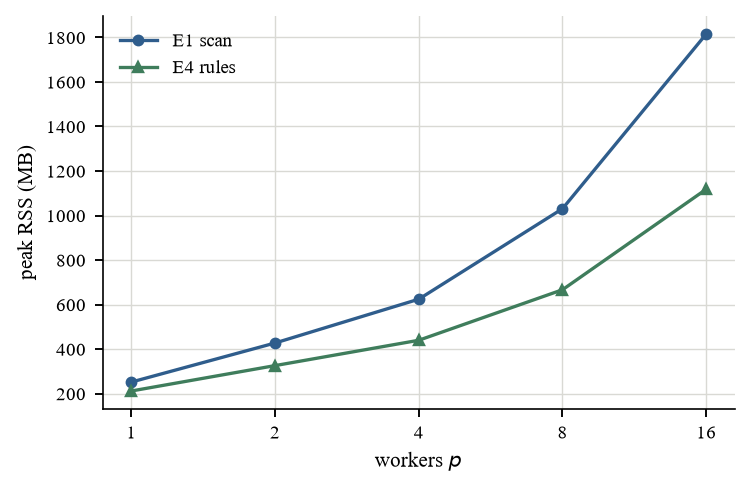
\includegraphics[width=\linewidth]{figures/fig13_memory.png}
\caption{Peak resident memory against worker count. Process-based parallelism duplicates interpreter and data structures per worker; beyond 8 workers the memory cost grows faster than the time saving on this machine.}
\end{figure}

\textbf{The memory cost of parallelism.} Figure 13 is the trade-off typically omitted. Every additional process duplicates the interpreter, the parsed shared structures and the per-worker buffers: 252 MB at one worker against 1815 MB at sixteen. On a workstation with 34 GB this is affordable; on the 8 GB laptops most students actually have, the same configuration would swap, and the wall-clock result would invert. Parallelism is not free, and the free resource is time only if memory is abundant.

% Discussion
% Generated by report/md2tex.py from Report.md -- edit Report.md, then re-run.

\section{Discussion}

\subsection{What the three tiers say together}

The four experiments are deliberately different in shape, and the comparison is the report's main technical claim: "parallelise it" is not one decision but three, and which one applies is determined by the workload's dependency structure, not by the hardware. A scan has no dependencies and scales until the serial merge bites. An iterative solver has one dependency per iteration and stops scaling when the iteration becomes shorter than the barrier. An irregular mining phase has data-dependent cost and stops scaling when the slowest shard determines the finish, which no amount of workers fixes. The same machine produced 6.93$\times$, 1.67$\times$ and 4.34$\times$ on three workloads of comparable size.

\subsection{An implementation defect worth reporting}

The first version of the scan tier created a fresh process pool for each of the four stages. Measured that way, the pipeline peaked at 2.62$\times$ at 4 workers and \emph{slowed down} at 16: the two smallest files spent more time spawning sixteen interpreters than parsing their contents, and the row-count-identical work took 63 s at 16 workers against 42 s at 4. Reusing one pool across all four stages, and spilling the read-only reference set to disk so each worker loads it once instead of receiving it with every chunk task, raised the same measurement to 6.93$\times$ at 16 workers. The defect was invisible in the algorithmic analysis and only appeared because the benchmark reported per-stage timings rather than one total: the large stage was scaling fine while the small ones were going backwards.

\subsection{Bottlenecks}

Three bottlenecks were predicted in the proposal and all three were confirmed. The serial gunzip (33.8 s) caps the end-to-end benefit of every later stage; the parent-side merge caps the scan tier; and the inter-iteration barrier caps PageRank. A fourth was not predicted: process-based parallelism multiplies memory, which is the binding constraint on the hardware this project targets. A fifth is a property of the machine rather than of the algorithm: the 16-worker configuration exceeds the 14 physical cores, and eight of those cores are efficiency cores with roughly half the throughput of the performance cores. Work split evenly by count is therefore not split evenly by time, and the slowest worker sets the finish. The 43\% efficiency at 16 workers consequently mixes two effects \textemdash{} the serial merge and heterogeneous core placement \textemdash{} and this experiment does not attempt to separate them.

\subsection{Threats to validity}

\textbf{The working set is a release market, not an industry.} As Section 4.1 documents, no field in this release identifies a production country, and the three definitions we tested select 25,997, 15,715 or 0 titles. The analysis is therefore about films released in Hong Kong, and statements about "the local industry" refer to the Cantonese-language bloc identified in Section 4.3, not to a curated list of Hong Kong productions. Any claim about market share or output volume would inherit this error; claims about network structure within a bloc are less exposed, because bloc membership is itself estimated from the collaboration data.

\textbf{Billing truncation.} Taking the eight top-billed acting credits per title systematically drops unbilled supporting players and background performers, whose absence inflates the apparent density of the core. We report results at top-3 and top-8 as a sensitivity check; the bloc structure is stable between them, but node counts differ by a factor of 2.4 (21,912 versus 51,878), so no absolute density or degree figure should be read as a property of the industry rather than of the truncation rule.

\textbf{IMDb coverage.} Cast lists are incomplete for pre-1970 films and for Cantonese productions whose credits were never transcribed. The pre-1980 peak in Figure 3 is partly a cataloguing artefact, and the 1980s trough is almost certainly one. Temporal conclusions are therefore stated as within-sample trends, not as industry history.

\textbf{Sampling in betweenness.} With 64 pivots the ranking of the top 50 nodes is preserved against a 256-pivot run, but individual scores carry sampling error and are reported only as ranks, never as magnitudes.

% Conclusion and Future Work
% Generated by report/md2tex.py from Report.md -- edit Report.md, then re-run.

\section{Conclusion and Future Work}

Three claims are supported. Substantively, the Hong Kong release network decomposes into cinema blocs that an unsupervised algorithm recovers from co-appearance alone, at modularity 0.75 and with cross-seed stability 0.89, and the local Cantonese-language bloc is identifiable by the people the industry's own histories name as its core. Methodologically, three parallel strategies applied to three workload shapes on one machine produce three different ceilings \textemdash{} 6.93$\times$, 1.67$\times$, 4.34$\times$ \textemdash{} and the differences are explained by dependency structure and memory hierarchy before they are measured. Practically, a workstation-scale implementation with process-level parallelism and cache-aware blocking captures most of the available gain for the scan and counting tiers, and should not be applied to the iterative tier at this graph size.

Future work, in the order we would attempt it: replace Apriori's candidate generation with FP-Growth and re-measure E4, which should move the ceiling from the irregular phase to the counting phase; obtain a country-of-origin label from a source that has one \textemdash{} Wikidata was unreachable from the test environment, but a bulk dump would remove the largest threat to validity; extend the temporal analysis from fixed-label profiles to a genuinely dynamic community method; and test whether bloc position predicts commercial outcomes once box-office data is joined.

% Individual Contribution Statement
% Generated by report/md2tex.py from Report.md -- edit Report.md, then re-run.

\section{Individual Contribution Statement}

\begin{table}[H]
\centering
\footnotesize
\begin{tabularx}{\textwidth}{lXX}
\toprule
Member & Contribution & Share \\
\midrule
{}[Student Name 1] & Data acquisition and validation; S1 pipeline; E1 and E1b experiments; scaling harness & 27\% \\
{}[Student Name 2] & S2 graph construction; PageRank and Louvain implementations; E3 experiment & 27\% \\
{}[Student Name 3] & S4 rule mining; career clustering; figures 3\textendash{}9 and 14 & 26\% \\
{}[Student Name 4] & Report writing; figure standardisation; slide deck; Q\&A preparation & 20\% \\
\bottomrule
\end{tabularx}
\end{table}

% References
% Generated by report/md2tex.py from Report.md -- edit Report.md, then re-run.

\section{References}

\begin{enumerate}
  \item Page, L., Brin, S., Motwani, R., Winograd, T. (1999). The PageRank citation ranking: bringing order to the web. \emph{Stanford InfoLab Technical Report}.
  \item Blondel, V. D., Guillaume, J.-L., Lambiotte, R., Lefebvre, E. (2008). Fast unfolding of communities in large networks. \emph{Journal of Statistical Mechanics}, P10008.
  \item Zhu, X., Ghahramani, Z. (2002). Learning from labeled and unlabeled data with label propagation. \emph{CMU Technical Report}.
  \item Brandes, U. (2001). A faster algorithm for betweenness centrality. \emph{Journal of Mathematical Sociology}, 25(2), 163\textendash{}177.
  \item Agrawal, R., Srikant, R. (1994). Fast algorithms for mining association rules. \emph{Proc. VLDB}, 487\textendash{}499.
  \item Han, J., Pei, J., Yin, Y. (2000). Mining frequent patterns without candidate generation. \emph{Proc. SIGMOD}, 1\textendash{}12.
  \item Newman, M. E. J. (2006). Modularity and community structure in networks. \emph{PNAS}, 103(23), 8577\textendash{}8582.
  \item Dean, J., Ghemawat, S. (2008). MapReduce: simplified data processing on large clusters. \emph{CACM}, 51(1), 107\textendash{}113.
  \item Fortunato, S., Barth\'{e}lemy, M. (2007). Resolution limit in community detection. \emph{PNAS}, 104(1), 36\textendash{}41.
  \item Watts, D. J., Strogatz, S. H. (1998). Collective dynamics of small-world networks. \emph{Nature}, 393, 440\textendash{}442.
\end{enumerate}

% Appendix A. Reproducibility
% Generated by report/md2tex.py from Report.md -- edit Report.md, then re-run.

\section{Appendix A. Reproducibility}

\begin{verbatim}
Project_Work/
  src/download_data.py   segmented parallel fetch of the five dumps
  src/s1_scan.py         byte-range chunk scanner (the parallel primitive)
  src/pipeline.py        S0/S1 driver, writes the working set
  src/s2_graph.py        cast expansion and edge construction
  src/s3_analytics.py    PageRank, Louvain, label propagation, betweenness
  src/s4_rules.py        Apriori with sharded counting
  src/bench.py           E1, E1b, E3, E3b, E4 and the scaling sweeps
  src/analyze.py         substantive analysis, writes results/analysis.json
  src/figures.py         all figures, regenerated from results/
  results/*.jsonl        one line per benchmark run
\end{verbatim}

Every number in Section 4.6 is regenerated by \texttt{python src/bench.py --exp all}; every figure by \texttt{python src/figures.py}. Row counts are recorded in \texttt{results/s1\_summary.json} at the time of download.


\end{document}
